% answers.tex —— 2015 年·天津卷·理科 · 参考答案与详细解析片段
% 由 tools/generate_projects.py 依来源总账自 2015/2015_数学真题_天津理_试题.md + 2015/2015_数学真题_天津理_解析正文.md + 2015/2015_数学真题_天津理_答案要点.md 生成，勿手改（改源 MD 后重跑）

\begin{gktip}
固定原卷不附参考答案（等级 D），以下为逐题独立推导、逐题校验的解析（非官方答案）。第 3 题框图按源复刻（翻倍型 \(S=20,i=1\)／\(i=2i\)／\(i>5?\)，与常见 \(i=i+1\) 变体不同，见试题文件存疑 ②）；第 5 题的四个选项在源中排于栏 2 之首（断栏排版），本库按题归并；第 14 题系数为 \(\dfrac{1}{9\lambda}\)（照源）；第 19 题 (3) 按题面字面取两支之\textbf{并}（若命题本意限于第二象限则缩为 \(\left(-\infty,-\dfrac{2\sqrt{3}}{3}\right)\)，见该题末存疑登记）；第 20 题 (1) 的单调性须分 \(n\) 的奇偶讨论。
\end{gktip}

\begin{answer}
\gksolhead{1}{}

\textbf{题目}：

已知全集 \(U=\{1,2,3,4,5,6,7,8\}\)，集合 \(A=\{2,3,5,6\}\)，集合 \(B=\{1,3,4,6,7\}\)，则集合 \(A\cap\complement_U B=\)（　）

(A) \(\{2,5\}\)　(B) \(\{3,6\}\)　(C) \(\{2,5,6\}\)　(D) \(\{2,3,5,6,8\}\)

\Needspace{4\baselineskip}
\textbf{解析}

\Needspace{5\baselineskip}
由补集定义，全集 \(U=\{1,2,3,4,5,6,7,8\}\) 中不属于 \(B=\{1,3,4,6,7\}\) 的元素为 \(2,5,8\)，于是

\nopagebreak[4]
\[
\complement_U B=\{2,5,8\},\qquad A\cap\complement_U B=\{2,3,5,6\}\cap\{2,5,8\}=\{2,5\}.
\]

故选 (A)。

（验证：由恒等式 \(A\cap\complement_U B=A\setminus B\) 复核，即从 \(A=\{2,3,5,6\}\) 中删去属于 \(B\) 的元素 \(3,6\)，余下 \(\{2,5\}\)；再逐元素枚举 \(A\) 的四个元素——\(2\notin B\)、\(3\in B\)、\(5\notin B\)、\(6\in B\)，过筛后同为 \(\{2,5\}\)，两路一致。反向检验选项 (B) \(\{3,6\}\)：元素 \(3,6\) 都在 \(B\) 中，必不属于 \(\complement_U B\)，可直接排除。）

\gkanswer{答案：A（\(\{2,5\}\)）}

\end{answer}
\begin{answer}
\gksolhead{2}{}

\textbf{题目}：

设变量 \(x\)，\(y\) 满足约束条件 \(\begin{cases}x+2\geqslant0,\\x-y+3\geqslant0,\\2x+y-3\leqslant0,\end{cases}\) 则目标函数 \(z=x+6y\) 的最大值为（　）

(A) 3　(B) 4　(C) 18　(D) 40

\Needspace{4\baselineskip}
\textbf{解析}

三条边界为 \(x=-2\)、\(y=x+3\)、\(y=3-2x\)，可行域是 \(x\geqslant-2\) 与 \(y\leqslant x+3\)、\(y\leqslant 3-2x\) 的公共部分。由 \(x+3\leqslant 3-2x\iff x\leqslant 0\) 知：当 \(-2\leqslant x\leqslant 0\) 时上方边界为 \(y=x+3\)，当 \(x\geqslant 0\) 时上方边界为 \(y=3-2x\)。

目标函数 \(z=x+6y\) 对 \(y\) 单调递增，故最大值必在上方边界取得，分两段计算。

\Needspace{5\baselineskip}
第一段（\(-2\leqslant x\leqslant 0\)，上方边界 \(y=x+3\)）：

\nopagebreak[4]
\[
z=x+6(x+3)=7x+18\leqslant 18,
\]

\Needspace{5\baselineskip}
等号在 \(x=0\) 时成立。第二段（\(x\geqslant 0\)，上方边界 \(y=3-2x\)）：

\nopagebreak[4]
\[
z=x+6(3-2x)=18-11x\leqslant 18,
\]

等号同样在 \(x=0\) 时成立。故 \(z_{\max}=18\)，在点 \((0,3)\) 取得（代回三式：\(0+2\geqslant 0\)、\(0-3+3\geqslant 0\)、\(0+3-3\leqslant 0\) 均成立）。

故选 (C)。

（验证：三组边界两两求交得三个候选顶点，其中 \(x=-2\) 与 \(y=3-2x\) 的交点 \((-2,7)\) 不可行——代回 \(x-y+3=-2-7+3=-6<0\)，舍去；余下 \((-2,1)\)、\((0,3)\) 均可行，代入目标函数得 \(z(-2,1)=-2+6=4\)、\(z(0,3)=0+18=18\)。另对可行域做 20 万点随机采样，数值最大 \(z\approx 17.66\)，始终逼近而不超过 \(18\)，与逐段线性式的端点结论一致。）

\gkanswer{答案：C（\(18\)）}

\end{answer}
\begin{answer}
\gksolhead{3}{}

\textbf{题目}：

阅读程序框图，运行相应的程序，则输出 \(S\) 的值为（　）
\nopagebreak[4]
\begin{center}% ============================================================
% f2015tjl_q03_flowchart.tex —— 2015 天津卷（理科）第 3 题 程序框图
% ------------------------------------------------------------
% 坐标口径：图内画布 pt，原点 = 源页基准点，x 右正、y 上正。
%   来源：.work/phase3-b11/figure-inventory.md（真实页 pt，原点左上、y 向下）
%   换算：X_tikz = x_page − 179.30 ；  Y_tikz = 533.77 − y_page
% 线宽：图形本体 0.398 pt（清单 §1.2）。
% 箭头：TikZ arrows.meta 标准箭矢（> = Triangle），箭尖落于清单所给尖端坐标；
%       源图线段本体短于尖端（留白由填充三角补齐），TikZ 由 tip 自动收尾，等效。
% 标签：绝对字号 10.5pt / 行距 12.6pt，inner sep=0（全库既定，勿改相对字号）。
% 要素：7 框 + 6 主干 + 1 回折 = 14 描边 path；7 填充箭头（清单 §1.5 合计 21）。
% ============================================================
\usetikzlibrary{arrows.meta}
\begin{tikzpicture}[
  x=1pt,y=1pt,                             % 画布单位 = 1 pt（本文件坐标一律为 pt）
  every node/.style={font=\fontsize{10.5pt}{12.6pt}\selectfont,inner sep=0pt},
  >={Triangle[length=3.60pt,width=3.36pt]},
  fr/.style={line width=0.398pt},          % 框体
  ln/.style={line width=0.398pt},          % 主干 / 回折线
]

  % ---------- 主干线（x = 216.22 → 36.92；起笔点在段首，箭尖在段尾）----------
  \draw[ln,->] (36.92,184.78) -- (36.92,170.61);   % a 开始 → S=20,i=1
  \draw[ln,->] (36.92,154.01) -- (36.92,139.84);   % b S=20,i=1 → i=2i
  \draw[ln,->] (36.92,125.52) -- (36.92,111.34);   % c i=2i → S=S−i
  \draw[ln,->] (36.92, 95.89) -- (36.92, 81.72);   % d S=S−i → 菱形
  \draw[ln,->] (36.92, 62.82) -- (36.92, 48.64);   % e 菱形下顶点 → 输出 S
  \draw[ln,->] (36.92, 31.38) -- (36.92, 17.21);   % f 输出 S → 结束

  % ---------- 「否」支回折（3 段：右 → 上 → 左），自菱形右顶点右侧 0.28 起笔 ----------
  \draw[ln,->] (74.13,72.27) -- (88.31,72.27) -- (88.31,146.93) -- (36.92,146.93);

  % ---------- 节点框 ----------
  % 1 开始（圆角矩形，r≈3.99）
  \draw[fr,rounded corners=3.99pt] (22.92,184.98) rectangle (50.92,201.82);
  \node at (36.90,193.97) {开始};
  % 2 S=20, i=1
  \draw[fr] (3.01,154.21) rectangle (70.84,170.41);
  \node at (36.925,162.31) {$S=20,\,i=1$};
  % 3 i=2i
  \draw[fr] (20.18,125.72) rectangle (53.67,139.64);
  \node at (36.925,132.68) {$i=2i$};
  % 4 S=S−i
  \draw[fr] (11.15,96.09) rectangle (62.69,111.14);
  \node at (36.92,103.615) {$S=S-i$};
  % 5 i>5?（菱形，右/上/左/下顶点）
  \draw[fr] (73.85,72.27) -- (36.92,81.44) -- (0.00,72.27) -- (36.92,63.10) -- cycle;
  \node at (36.92,72.27) {$i>5?$};
  % 6 输出 S（非直角平行四边形，顶部右斜 6.14）
  \draw[fr] (11.51,31.58) -- (17.65,48.44) -- (62.33,48.44) -- (56.19,31.58) -- cycle;
  \node at (36.92,40.01) {输出 $S$};
  % 7 结束（圆角矩形，r≈3.99）
  \draw[fr,rounded corners=3.99pt] (22.92,0.00) rectangle (50.92,17.01);
  \node at (36.90,9.07) {结束};

  % ---------- 支标（清单 §1.4 实测字形中心）----------
  \node at (45.90,56.37) {是};
  \node at (74.10,64.57) {否};

\end{tikzpicture}
\end{center}
\nopagebreak[4]
(A) \(-10\)　(B) 6　(C) 14　(D) 18

\Needspace{4\baselineskip}
\textbf{解析}

框图流程：开始 → \(S=20,\ i=1\) → \(i=2i\) → \(S=S-i\) → 判 \(i>5\)？（否→回 \(i=2i\)；是→输出 \(S\) → 结束）。

逐步运行：初值 \(S=20\)、\(i=1\)。第 1 轮，\(i=2i=2\)，\(S=20-2=18\)，判断 \(2>5\) 不成立；第 2 轮，\(i=2\times2=4\)，\(S=18-4=14\)，判断 \(4>5\) 不成立；第 3 轮，\(i=2\times4=8\)，\(S=14-8=6\)，判断 \(8>5\) 成立，输出 \(S=6\)。

故选 (B)。

（验证：按框图逐轮模拟，\(S\) 的序列为 \(20\to18\to14\to6\)、\(i\) 的序列为 \(1\to2\to4\to8\)，第三轮 \(i=8>5\) 触发输出，与逐轮手算一致。再核对回跳位置：放大图中「否」支箭头自菱形右顶点右行、上折、再左折，汇入 \(i=2i\) 框顶，即回跳后重做 \(i=2i\)；若误读为回跳至 \(S=S-i\)，则 \(i\) 不再翻倍、判断 \(i>5\) 永不成立，与输出 \(6\) 明显分道（选项 (A) 的 \(-10\) 即该方向的干扰项），故取 \(6\)。）

\gkanswer{答案：B（\(6\)）}

\end{answer}
\begin{answer}
\gksolhead{4}{}

\textbf{题目}：

设 \(x\in\mathbf{R}\)，则“\(|x-2|<1\)”是“\(x^2+x-2>0\)”的（　）

(A) 充分而不必要条件　(B) 必要而不充分条件

(C) 充要条件　(D) 既不充分也不必要条件

\Needspace{4\baselineskip}
\textbf{解析}

\Needspace{5\baselineskip}
两个条件分别解出：

\nopagebreak[4]
\[
|x-2|<1\iff -1<x-2<1\iff 1<x<3,
\]

\nopagebreak[4]
\[
x^2+x-2>0\iff (x+2)(x-1)>0,
\]

即 \(x<-2\) 或 \(x>1\)。

充分性：由 \(1<x<3\) 必有 \(x>1\)，从而 \(x^2+x-2>0\) 成立，充分性成立。

必要性：取 \(x=5\)，此时 \(x^2+x-2=25+5-2=28>0\) 成立，但 \(|5-2|=3\)，不满足 \(|x-2|<1\)，必要性不成立。

故选 (A)。

（验证：从集合包含看，条件集 \(P=(1,3)\) 与结论集 \(Q=(-\infty,-2)\cup(1,+\infty)\) 满足 \(P\subsetneq Q\)，真包含即「充分而不必要」。反例单证必要性：\(x=5\) 时 \(25+5-2=28>0\) 而 \(|5-2|=3\) 不小于 \(1\)；正例复核充分性：\(x=2\) 时 \(|2-2|=0<1\) 与 \(4+2-2=4>0\) 同真。）

\gkanswer{答案：A（充分而不必要条件）}

\end{answer}
\begin{answer}
\gksolhead{5}{}

\textbf{题目}：

如图，在圆 \(O\) 中，\(M\)，\(N\) 是弦 \(AB\) 的三等分点，弦 \(CD\)，\(CE\) 分别经过点 \(M\)，\(N\)，若 \(CM=2\)，\(MD=4\)，\(CN=3\)，则线段 \(NE\) 的长为（　）
\nopagebreak[4]
\begin{center}% ============================================================
% f2015tjl_q05_circle.tex —— 2015 天津卷（理科）第 5 题 圆与割线
% ------------------------------------------------------------
% 坐标口径：图内画布 pt，原点 = 源页基准点，x 右正、y 上正。
%   来源：.work/phase3-b11/figure-inventory.md（真实页 pt，原点左上、y 向下）
%   换算：X_tikz = x_page − 169.40 ；  Y_tikz = 773.78 − y_page
% 线宽：圆 0.398 pt；弦 AB 0.398 pt（图形本体档，清单未单独标注，取本体档）；
%       两割线 CE / CD **0.42 pt**（清单 §2.3 实测值，源图自身与他线不同档，照源保留）。
% 照源复刻（清单 §7 存疑）：
%   S-3 圆心实心点为**字形** U+2022（\textbullet），非矢量填充；与「O」并置为「•O」，
%       字形落于文字基线，其墨迹中心较几何圆心 (53.895,53.890) 有约 3.6 pt 垂直偏置。
%   S-4 两割线在弦高 y=736.90 处与三等分点 M/N 有 1.65 / 0.49 pt 微差（源图未精确
%       满足题设交点约束）——**照源复刻，不「修正」**。
% 要素：3 描边 path（圆 / 弦 / 两割线合一）+ 8 文字标签（清单 §2.6）。
% ============================================================
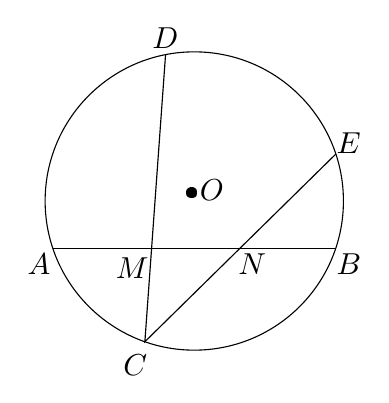
\begin{tikzpicture}[
  x=1pt,y=1pt,                             % 画布单位 = 1 pt（本文件坐标一律为 pt）
  every node/.style={font=\fontsize{10.5pt}{12.6pt}\selectfont,inner sep=0pt},
  body/.style={line width=0.398pt},
  sec/.style={line width=0.420pt},
]

  % ---------- 圆（圆心 (223.295,719.890)，r = 53.895）----------
  \draw[body] (53.895,53.890) circle [radius=53.895pt];

  % ---------- 弦 AB（水平全长弦，(172.10,736.90)→(274.50,736.90)，长 102.40）----------
  \draw[body] (2.70,36.88) -- (105.10,36.88);

  % ---------- 两割线（源图为 1 个 path 的 2 个子段，共点 C）----------
  % CE：E(274.49,702.88) → C(205.44,770.75)
  % CD：C(205.44,770.75) → D(212.92,666.99)
  \draw[sec] (105.09,70.90) -- (36.04,3.03) -- (43.52,106.79);

  % ---------- 标签（清单 §2.5 实测字形中心）----------
  \node at (-2.20,30.98)  {$A$};
  \node at (109.80,30.98) {$B$};
  \node at (32.60,-5.32)  {$C$};
  \node at (43.40,112.78) {$D$};
  \node at (109.70,74.88) {$E$};
  \node at (31.50,29.58)  {$M$};
  \node at (74.80,30.98)  {$N$};

  % ---------- 圆心「•O」：U+2022 字形与 O 并置（S-3 照源）----------
  \node at (57.495,57.86) {\textbullet $O$};

\end{tikzpicture}
\end{center}
\nopagebreak[4]
(A) \(\dfrac{8}{3}\)　(B) 3　(C) \(\dfrac{10}{3}\)　(D) \(\dfrac{5}{2}\)

\Needspace{4\baselineskip}
\textbf{解析}

设 \(AM=MN=NB=t\)，则 \(MB=2t\)、\(AN=2t\)、\(NB=t\)。

\Needspace{5\baselineskip}
\(M\) 是弦 \(AB\) 与 \(CD\) 的交点，由相交弦定理得

\nopagebreak[4]
\[
CM\cdot MD=AM\cdot MB=t\cdot 2t=2t^2,
\]

代入 \(CM=2\)、\(MD=4\)，得 \(8=2t^2\)，即 \(t^2=4\)。

\Needspace{5\baselineskip}
\(N\) 是弦 \(AB\) 与 \(CE\) 的交点，再由相交弦定理得

\nopagebreak[4]
\[
CN\cdot NE=AN\cdot NB=2t\cdot t=2t^2=8,
\]

代入 \(CN=3\)，得 \(3\cdot NE=8\)，故 \(NE=\dfrac{8}{3}\)。

故选 (A)。

（验证：路线一在 \(M\) 处定参——\(CM\cdot MD=2\times 4=8=2t^2\)，回代 \(N\) 处 \(2t^2=8\)，得 \(NE=\dfrac{8}{3}\)。路线二以坐标独立复算：取 \(A(-3,0)\)、\(M(-1,0)\)、\(N(1,0)\)、\(B(3,0)\)（即 \(t=2\) 的构型），由 \(CM=2\)、\(CN=3\) 相减解出 \(C\) 的横坐标为 \(-\dfrac{5}{4}\)；作过 \(A,B,C\) 的圆，其与直线 \(CN\) 的第三个交点 \(E\) 算得与 \(N\) 的横向差为 \(2\)、纵向差为 \(\dfrac{2\sqrt{7}}{3}\)，故 \(NE=\sqrt{4+\dfrac{28}{9}}=\dfrac{8}{3}\)，与路线一吻合；回代验证 \(E\) 在圆上——到圆心的距离平方 \(9+\dfrac{7}{9}=\dfrac{88}{9}\) 恰等于半径平方，两路一致。）

\gkanswer{答案：A（\(\dfrac{8}{3}\)）}

\end{answer}
\begin{answer}
\gksolhead{6}{}

\textbf{题目}：

已知双曲线 \(\dfrac{x^2}{a^2}-\dfrac{y^2}{b^2}=1\)（\(a>0\)，\(b>0\)）的一条渐近线过点 \((2,\sqrt{3})\)，且双曲线的一个焦点在抛物线 \(y^2=4\sqrt{7}x\) 的准线上，则双曲线的方程为（　）

(A) \(\dfrac{x^2}{21}-\dfrac{y^2}{28}=1\)　(B) \(\dfrac{x^2}{28}-\dfrac{y^2}{21}=1\)

(C) \(\dfrac{x^2}{3}-\dfrac{y^2}{4}=1\)　(D) \(\dfrac{x^2}{4}-\dfrac{y^2}{3}=1\)

\Needspace{4\baselineskip}
\textbf{解析}

\Needspace{5\baselineskip}
双曲线的渐近线为 \(y=\pm\dfrac{b}{a}x\)。点 \((2,\sqrt{3})\) 在第一象限，故它只落在渐近线 \(y=\dfrac{b}{a}x\) 上，代入得 \(\dfrac{b}{a}\times 2=\sqrt{3}\)，即

\nopagebreak[4]
\[
\dfrac{b^2}{a^2}=\dfrac{3}{4}.
\]

\Needspace{5\baselineskip}
抛物线 \(y^2=4\sqrt{7}x\) 中 \(2p=4\sqrt{7}\)，故 \(p=2\sqrt{7}\)，准线为 \(x=-\dfrac{p}{2}=-\sqrt{7}\)。双曲线焦点为 \((\pm c,0)\)，其中 \(c=\sqrt{a^2+b^2}\)，由一个焦点落在准线上得 \(c=\sqrt{7}\)，即

\nopagebreak[4]
\[
a^2+b^2=7.
\]

\Needspace{5\baselineskip}
联立 \(b^2=\dfrac{3}{4}a^2\) 与 \(a^2+b^2=7\)，得 \(\dfrac{7}{4}a^2=7\)，故 \(a^2=4\)、\(b^2=3\)，所求方程为

\nopagebreak[4]
\[
\dfrac{x^2}{4}-\dfrac{y^2}{3}=1.
\]

故选 (D)。

（验证：对四个选项同时回代两个条件，其中渐近线条件等价于 \(\dfrac{b^2}{a^2}=\dfrac{3}{4}\)，焦点条件等价于 \(a^2+b^2=7\)。(A) \(a^2=21\)、\(b^2=28\)：\(\dfrac{b^2}{a^2}=\dfrac{4}{3}\) 且 \(a^2+b^2=49\)，双条皆不合；(B) \(a^2=28\)、\(b^2=21\)：\(\dfrac{b^2}{a^2}=\dfrac{3}{4}\) 合渐近线，而 \(a^2+b^2=49\) 不合焦点；(C) \(a^2=3\)、\(b^2=4\)：\(\dfrac{b^2}{a^2}=\dfrac{4}{3}\) 不合渐近线，而 \(a^2+b^2=7\) 合焦点；(D) \(a^2=4\)、\(b^2=3\)：\(\dfrac{b^2}{a^2}=\dfrac{3}{4}\)、\(a^2+b^2=7\)，双条全过。仅 (D) 同时满足。另核对陷阱：\(y^2=4\sqrt{7}x\) 的准线为 \(x=-\sqrt{7}\)，若误按 \(x=-p\) 计算会得 \(c^2=28\)，进而得 \(a^2=16\)、\(b^2=12\)，该方程不在选项中，正是排除此误读的判别点。）

\gkanswer{答案：D（\(\dfrac{x^2}{4}-\dfrac{y^2}{3}=1\)）}

\end{answer}
\begin{answer}
\gksolhead{7}{}

\textbf{题目}：

已知定义在 \(\mathbf{R}\) 上的函数 \(f(x)=2^{|x-m|}-1\)（\(m\) 为实数）为偶函数，记 \(a=f(\log_{0.5}3)\)，\(b=f(\log_2 5)\)，\(c=f(2m)\)，则 \(a\)，\(b\)，\(c\) 的大小关系为（　）

(A) \(a<b<c\)　(B) \(a<c<b\)　(C) \(c<a<b\)　(D) \(c<b<a\)

\Needspace{4\baselineskip}
\textbf{解析}

\Needspace{5\baselineskip}
\(f(x)\) 为偶函数，故对任意 \(x\) 有 \(f(-x)=f(x)\)，即 \(2^{|-x-m|}=2^{|x-m|}\)，从而 \(|x+m|=|x-m|\) 恒成立。取 \(x=m\) 得 \(|2m|=0\)，故 \(m=0\)，于是

\nopagebreak[4]
\[
f(x)=2^{|x|}-1.
\]

\Needspace{5\baselineskip}
逐项求值：

\nopagebreak[4]
\[
a=f(\log_{0.5}3)=f(-\log_2 3)=2^{\log_2 3}-1=3-1=2,
\]

\nopagebreak[4]
\[
b=f(\log_2 5)=2^{\log_2 5}-1=5-1=4,
\]

\nopagebreak[4]
\[
c=f(2m)=f(0)=2^0-1=0.
\]

故 \(c<a<b\)。

故选 (C)。

（验证：三条取值均为精确整数，不含任何近似——\(a=3-1=2\)、\(b=5-1=4\)、\(c=1-1=0\)，其序 \(0<2<4\) 即 \(c<a<b\)。另用单调性互证：\(f(x)=2^{|x|}-1\) 随 \(|x|\) 递增，而 \(|-\log_2 3|=\log_2 3\approx 1.585\)、\(\log_2 5\approx 2.322\)、\(|0|=0\)，序 \(0<1.585<2.322\) 与函数值序 \(0<2<4\) 一致。选项 (B) \(a<c<b\) 为易混项——此处 \(c=0\) 取的是最小值而非居中值，故取 (C)。）

\gkanswer{答案：C（\(c<a<b\)）}

\end{answer}
\begin{answer}
\gksolhead{8}{}

\textbf{题目}：

已知函数 $f(x)=\begin{cases}2-|x|,&x\leqslant2,\\(x-2)^2,&x>2,\end{cases}$ 函数 \(g(x)=b-f(2-x)\)，其中 \(b\in\mathbf{R}\)．若函数 \(y=f(x)-g(x)\) 恰有 4 个零点，则 \(b\) 的取值范围是（　）

(A) \(\left(\dfrac{7}{4},+\infty\right)\)　(B) \(\left(-\infty,\dfrac{7}{4}\right)\)　(C) \(\left(0,\dfrac{7}{4}\right)\)　(D) \(\left(\dfrac{7}{4},2\right)\)

\Needspace{4\baselineskip}
\textbf{解析}

\Needspace{5\baselineskip}
零点方程等价变形：

\nopagebreak[4]
\[
y=f(x)-g(x)=0\iff f(x)=b-f(2-x)\iff f(x)+f(2-x)=b.
\]

记 \(h(x)=f(x)+f(2-x)\)，问题化为方程 \(h(x)=b\) 恰有 4 个解。

按 \(x\) 所在区间分段求出 \(h\)：

当 \(0\leqslant x\leqslant 2\) 时，\(2-x\in[0,2]\)，有 \(f(x)=2-x\)、\(f(2-x)=2-(2-x)=x\)，故 \(h(x)\equiv 2\)；

当 \(x>2\) 时，\(2-x<0\)，有 \(f(x)=(x-2)^2\)、\(f(2-x)=2-|2-x|=2-(x-2)=4-x\)，故 \(h(x)=(x-2)^2-x+4\)，令 \(u=x-2>0\)，得 \(h=u^2-u+2=\left(u-\dfrac{1}{2}\right)^2+\dfrac{7}{4}\geqslant\dfrac{7}{4}\)，等号当 \(u=\dfrac{1}{2}\)（即 \(x=\dfrac{5}{2}\)）时成立，且 \(u\to 0^+\) 时 \(h\to 2\)；

当 \(x<0\) 时，\(2-x>2\)，有 \(f(x)=2-|x|=2+x\)、\(f(2-x)=(2-x-2)^2=x^2\)，故 \(h(x)=x^2+x+2=\left(x+\dfrac{1}{2}\right)^2+\dfrac{7}{4}\geqslant\dfrac{7}{4}\)，等号当 \(x=-\dfrac{1}{2}\) 时成立，且 \(x\to 0^-\) 时 \(h\to 2\)。

逐段统计解的个数：

当 \(b<\dfrac{7}{4}\) 时，三段均无解，共 0 个；

当 \(b=\dfrac{7}{4}\) 时，左段得 \(x=-\dfrac{1}{2}\)，右段得 \(x=\dfrac{5}{2}\)，共 2 个；

当 \(\dfrac{7}{4}<b<2\) 时，左段方程 \(x^2+x+2=b\) 的两根分居 \(-\dfrac{1}{2}\) 两侧（均满足 \(x<0\)），右段方程 \(u^2-u+2=b\) 的两根分居 \(u=\dfrac{1}{2}\) 两侧（均给出 \(x>2\)），中段 \(h\equiv 2\) 无解，共 4 个；

当 \(b=2\) 时，左段得 \(x=-1\)，右段得 \(x=3\)，而中段 \([0,2]\) 上 \(h\equiv 2\)，整段都是解，解有无穷多个；

当 \(b>2\) 时，左段一根、右段一根，共 2 个。

故恰有 4 个零点当且仅当 \(\dfrac{7}{4}<b<2\)。

故选 (D)。

（验证：以 \(h(x)=f(x)+f(2-x)\) 在 \([-30,30]\) 上按细网格统计符号变化——\(b=1.5\) 得 0 个零点；\(b=1.8\)、\(1.9\)、\(1.999999\) 均得 4 个零点；\(b=2\) 在常值段 \([0,2]\) 上检出 6668 个网格零点（整段为解，印证「无穷多解」而非 4 解）；\(b=3\) 得 2 个零点。另数值复核两支的极小值 \(h(-0.5)=h(2.5)=1.75=\dfrac{7}{4}\)，且 \(h\) 在 \(x=0,0.5,1,1.5,2\) 处取值全为 \(2\)，与常值段结论一致。）

\gkanswer{答案：D（\(\left(\dfrac{7}{4},2\right)\)）}

\end{answer}
\begin{answer}
\gksolhead{9}{}

\textbf{题目}：

\(\mathrm{i}\) 是虚数单位，若复数 \((1-2\mathrm{i})(a+\mathrm{i})\) 是纯虚数，则实数 \(a\) 的值为\gkblank{}．

\Needspace{4\baselineskip}
\textbf{解析}

\Needspace{5\baselineskip}
展开所给复数：

\nopagebreak[4]
\[
(1-2\mathrm{i})(a+\mathrm{i})=a+\mathrm{i}-2a\mathrm{i}-2\mathrm{i}^2=(a+2)+(1-2a)\mathrm{i}.
\]

复数为纯虚数当且仅当实部为零且虚部不为零。由 \(a+2=0\) 得 \(a=-2\)，此时虚部为 \(1-2\times(-2)=5\neq0\)，条件满足。

所以实数 \(a\) 的值为 \(-2\)。

（验证：把 \(a=-2\) 回代得 \((1-2\mathrm{i})(-2+\mathrm{i})=5\mathrm{i}\)，为纯虚数；此时实部为 \(0\)、虚部为 \(5\)，纯虚数的两个条件均核对无误。）

\gkanswer{答案：\(-2\)}

\end{answer}
\begin{answer}
\gksolhead{10}{}

\textbf{题目}：

一个几何体的三视图如图所示（单位：m），则该几何体的体积为\gkblank{}m³．
\nopagebreak[4]
\begin{center}% ============================================================
% f2015tjl_q10_views.tex —— 2015 天津卷（理科）第 10 题 三视图
% ------------------------------------------------------------
% 坐标口径：图内画布 pt，原点 = 源页基准点，x 右正、y 上正。
%   来源：.work/phase3-b11/figure-inventory.md（真实页 pt，原点左上、y 向下）
%   换算：X_tikz = x_page − 493.36 ；  Y_tikz = 573.70 − y_page
% 比例基准：源题「1」= 28.35 pt（清单 §3），全图尺寸标注均为其整数倍。
% 线宽：图形本体 0.398 pt（轮廓 / 分隔线 / 尺寸线 / 界限短线统一本档）。
% 箭头：TikZ arrows.meta 标准箭矢（> = Triangle）；尺寸线每段一枚实心三角，
%       箭尖落在段尾坐标（= 清单所列「起点→终点」的终点，指向最近的尺寸界限线）。
% 照源复刻（清单 §7 存疑）：
%   S-5 俯视图**无水平尺寸线**（正视图有「1 | 2 | 1」三条）——不补。
%   S-6 侧视图半径线本体止于 (196.09,159.24)，箭尖 (198.63,161.78) 至圆心 28.35 = 恰好 1 图；
%       「线段长」与「半径」口径不一致——照源，半径以尖端计。
% 要素：46 描边 path（正视 27 + 侧视 2 + 俯视 17）+ 23 填充箭头（14 + 1 + 8）
%       + 9 文字标签（清单 §3.5 B 表、§3.4）。
% ============================================================
\usetikzlibrary{arrows.meta}
\begin{tikzpicture}[
  x=1pt,y=1pt,                             % 画布单位 = 1 pt（本文件坐标一律为 pt）
  every node/.style={font=\fontsize{10.5pt}{12.6pt}\selectfont,inner sep=0pt},
  >={Triangle[length=3.60pt,width=3.36pt]},
  g/.style={line width=0.398pt},
]

  % =========================================================
  % 正视图（上左）
  % =========================================================
  % 轮廓（6 点六边形：中央 2 图×2 图矩形 + 左右各伸 1 图三角尖）
  \draw[g] (8.50,141.74) -- (36.85,113.39) -- (93.54,113.39) -- (121.89,141.74)
           -- (93.54,170.08) -- (36.85,170.08) -- cycle;
  % 内部分隔竖线
  \draw[g] (36.85,113.39) -- (36.85,170.08);
  \draw[g] (93.54,113.39) -- (93.54,170.08);
  % 尺寸箭头：竖直 · 右外 @ X=127.56（每组「1」上下各一枚，箭尖朝外）
  \draw[g,->] (127.56,121.89) -- (127.56,116.98);
  \draw[g,->] (127.56,133.23) -- (127.56,138.15);
  \draw[g,->] (127.56,150.24) -- (127.56,145.32);
  \draw[g,->] (127.56,161.58) -- (127.56,166.50);
  % 尺寸箭头：竖直 · 左外 @ X=2.83
  \draw[g,->] (2.83,121.89) -- (2.83,116.98);
  \draw[g,->] (2.83,133.23) -- (2.83,138.15);
  \draw[g,->] (2.83,150.24) -- (2.83,145.32);
  \draw[g,->] (2.83,161.58) -- (2.83,166.50);
  % 尺寸箭头：水平 · 下方 @ Y=107.72（三段读数 1 | 2 | 1）
  \draw[g,->] (17.00,107.72) -- (12.09,107.72);
  \draw[g,->] (28.34,107.72) -- (33.26,107.72);
  \draw[g,->] (59.52,107.72) -- (40.43,107.72);
  \draw[g,->] (70.86,107.72) -- (89.95,107.72);
  \draw[g,->] (102.04,107.72) -- (97.13,107.72);
  \draw[g,->] (113.38,107.72) -- (118.30,107.72);
  % 尺寸界限短线：左外 3 条 / 右外 3 条
  \draw[g] (5.67,113.39) -- (0.00,113.39);
  \draw[g] (5.67,141.74) -- (0.00,141.74);
  \draw[g] (5.67,170.08) -- (0.00,170.08);
  \draw[g] (124.72,113.39) -- (130.39,113.39);
  \draw[g] (124.72,141.74) -- (130.39,141.74);
  \draw[g] (124.72,170.08) -- (130.39,170.08);
  % 尺寸界限短线：下方竖短线 4 条 @ 轮廓四角 x
  \draw[g] (8.50,110.55)  -- (8.50,104.89);
  \draw[g] (36.85,110.55) -- (36.85,104.89);
  \draw[g] (93.54,110.55) -- (93.54,104.89);
  \draw[g] (121.89,110.55) -- (121.89,104.89);
  % 读数与图名
  \node at (22.64,107.00)  {1};
  \node at (65.24,107.00)  {2};
  \node at (107.74,107.00) {1};
  \node at (2.84,155.20)   {1};
  \node at (2.84,126.80)   {1};
  \node at (127.54,155.20) {1};
  \node at (127.54,126.80) {1};
  \node at (65.24,91.30)   {正视图};

  % =========================================================
  % 侧视图（上右）：半径 1 图圆 + 半径引导线
  % =========================================================
  \draw[g] (178.58,141.74) circle [radius=28.35pt];
  \draw[g,->] (178.58,141.74) -- (198.63,161.78);
  \node at (192.74,143.80) {1};
  \node at (178.54,91.30)  {侧视图};

  % =========================================================
  % 俯视图（下左）：与正视图同形同尺寸，沿 y 下移 113.39
  % =========================================================
  \draw[g] (8.50,28.35) -- (36.85,0.00) -- (93.54,0.00) -- (121.89,28.35)
           -- (93.54,56.70) -- (36.85,56.70) -- cycle;
  \draw[g] (36.85,0.00) -- (36.85,56.70);
  \draw[g] (93.54,0.00) -- (93.54,56.70);
  % 尺寸箭头：竖直 · 右外 @ X=127.56
  \draw[g,->] (127.56,8.51)  -- (127.56,3.59);
  \draw[g,->] (127.56,19.84) -- (127.56,24.76);
  \draw[g,->] (127.56,36.85) -- (127.56,31.93);
  \draw[g,->] (127.56,48.19) -- (127.56,53.11);
  % 尺寸箭头：竖直 · 左外 @ X=2.83
  \draw[g,->] (2.83,8.51)  -- (2.83,3.59);
  \draw[g,->] (2.83,19.84) -- (2.83,24.76);
  \draw[g,->] (2.83,36.85) -- (2.83,31.93);
  \draw[g,->] (2.83,48.19) -- (2.83,53.11);
  % 尺寸界限短线：左外 3 条 / 右外 3 条（照源无水平尺寸线，S-5）
  \draw[g] (5.67,0.00)  -- (0.00,0.00);
  \draw[g] (5.67,28.35) -- (0.00,28.35);
  \draw[g] (5.67,56.70) -- (0.00,56.70);
  \draw[g] (124.72,0.00)  -- (130.39,0.00);
  \draw[g] (124.72,28.35) -- (130.39,28.35);
  \draw[g] (124.72,56.70) -- (130.39,56.70);
  % 读数与图名
  \node at (2.84,41.80)   {1};
  \node at (2.84,13.40)   {1};
  \node at (127.54,41.80) {1};
  \node at (127.54,13.40) {1};
  \node at (65.24,-13.50) {俯视图};

\end{tikzpicture}
\end{center}
\nopagebreak[4]
\Needspace{4\baselineskip}
\textbf{解析}

由三视图读数还原几何体。正视图由左右两个三角形与中间一个矩形拼成：横向标注依次为 \(1\)、\(2\)、\(1\)（总宽 \(4\)），纵向标注为两个 \(1\)（总高 \(2\)），左右尖点都落在中线高度上；侧视图是半径为 \(1\) 的圆；俯视图与正视图同形同尺寸，纵向同样为两个 \(1\)（总进深 \(2\)）。

\Needspace{5\baselineskip}
取长轴为 \(x\) 轴，设垂直于长轴的截面是半径为 \(r(x)\) 的圆盘。侧视图为半径 \(1\) 的整圆盘，故各截面都是圆盘、最大半径为 \(1\)；正视图与俯视图的中段同时读满高 \(2\)、进深 \(2\)，即该段截面在纵横两个方向上都取到直径 \(2\)，只能是半径 \(1\) 的整圆盘；两端各以尖点收束（各占 \(1\)），故两端各接一个底面半径 \(1\)、高 \(1\) 的圆锥。于是

\nopagebreak[4]
\[
r(x)=\begin{cases}x+2,&-2\leqslant x\leqslant-1,\\1,&-1\leqslant x\leqslant1,\\2-x,&1\leqslant x\leqslant2.\end{cases}
\]

\Needspace{5\baselineskip}
即几何体是半径 \(1\)、长 \(2\) 的圆柱两端各拼接一个底面半径 \(1\)、高 \(1\) 的圆锥。

\nopagebreak[4]
\[
V=\pi\times1^2\times2+2\times\dfrac13\pi\times1^2\times1=2\pi+\dfrac{2\pi}3=\dfrac{8\pi}3.
\]

所以该几何体的体积为 \(\dfrac{8\pi}{3}\ \mathrm{m}^3\)。

（验证：按卡瓦列里原理把截面积 \(\pi r(x)^2\) 在 \(\left[-2,2\right]\) 上分 40 万段数值求和，得 \(8.3775804095\)，与解析值 \(\dfrac{8\pi}{3}=8.3775804096\) 的相对差约 \(6\times10^{-12}\)；三视图读数自洽：侧视图半径 \(1\) 与最大截面半径 \(1\) 一致，正视图横向的 \(1\)、\(2\)、\(1\) 与两端锥高 \(1\)、中段长 \(2\) 对应，中段的高 \(2\)、进深 \(2\) 与正视图、俯视图纵向的两个 \(1\) 一致；再把所得几何体沿长轴方向投影得半径 \(1\) 的圆盘、沿两个横向投影均得两端三角形夹矩形、总宽 \(4\)、总高 \(2\) 的图形，与三视图逐条吻合。）

\gkanswer{答案：\(\dfrac{8\pi}{3}\ \mathrm{m}^3\)}

\end{answer}
\begin{answer}
\gksolhead{11}{}

\textbf{题目}：

曲线 \(y=x^2\) 与直线 \(y=x\) 所围成的封闭图形的面积为\gkblank{}．

\Needspace{4\baselineskip}
\textbf{解析}

\Needspace{5\baselineskip}
两曲线交点由 \(x^2=x\) 解得 \(x=0\)、\(x=1\)；在 \((0,1)\) 内恒有 \(x>x^2\)，故所围封闭图形夹在两交点之间，直线在上、抛物线在下：

\nopagebreak[4]
\[
S=\int_0^1\left(x-x^2\right)dx=\dfrac12-\dfrac13=\dfrac16.
\]

所以该封闭图形的面积为 \(\dfrac16\)。

（验证：定积分的精确值为 \(\dfrac12-\dfrac13=\dfrac16=0.1666666667\)；对同一积分作 50 万段中点法数值积分得 \(0.1666666667\)，与精确值之差约 \(3\times10^{-13}\)；在 \((0,1)\) 内逐点核对 \(x>x^2\) 亦成立。）

\gkanswer{答案：\(\dfrac{1}{6}\)}

\end{answer}
\begin{answer}
\gksolhead{12}{}

\textbf{题目}：

在 \(\left(x-\dfrac{1}{4x}\right)^6\) 的展开式中，\(x^2\) 的系数为\gkblank{}．

\Needspace{4\baselineskip}
\textbf{解析}

\Needspace{5\baselineskip}
二项展开的通项为

\nopagebreak[4]
\[
T_{k+1}=\binom6k x^{6-k}\left(-\dfrac1{4x}\right)^k=\binom6k\left(-\dfrac14\right)^k x^{6-2k}\quad(k=0,1,\dots,6).
\]

\Needspace{5\baselineskip}
令 \(6-2k=2\) 得 \(k=2\)，故 \(x^2\) 的系数为

\nopagebreak[4]
\[
\binom62\left(\dfrac14\right)^2=15\times\dfrac1{16}=\dfrac{15}{16}.
\]

所以 \(x^2\) 的系数为 \(\dfrac{15}{16}\)。

（验证：把 \(\left(x-\dfrac1{4x}\right)^6\) 按六个因式连乘逐项全展开（分数精确运算），所得 \(x^2\) 系数仍为 \(\dfrac{15}{16}\)，与通项法一致；全展开的非零项为 \(x^{-6}\) 项系数 \(\dfrac1{4096}\)、\(x^{-4}\) 项系数 \(-\dfrac3{512}\)、\(x^{-2}\) 项系数 \(\dfrac{15}{256}\)、常数项 \(-\dfrac5{16}\)、\(x^4\) 项系数 \(-\dfrac32\)、\(x^6\) 项系数 \(1\)。）

\gkanswer{答案：\(\dfrac{15}{16}\)}

\end{answer}
\begin{answer}
\gksolhead{13}{}

\textbf{题目}：

在 \(\triangle ABC\) 中，内角 \(A\)，\(B\)，\(C\) 所对的边分别为 \(a\)，\(b\)，\(c\)．已知 \(\triangle ABC\) 的面积为 \(3\sqrt{15}\)，\(b-c=2\)，\(\cos A=-\dfrac{1}{4}\)，则 \(a\) 的值为\gkblank{}．

\Needspace{4\baselineskip}
\textbf{解析}

\Needspace{5\baselineskip}
由 \(\cos A=-\dfrac14<0\) 知 \(A\) 为钝角，故

\nopagebreak[4]
\[
\sin A=\sqrt{1-\cos^2A}=\sqrt{1-\left(\dfrac14\right)^2}=\dfrac{\sqrt{15}}4.
\]

\Needspace{5\baselineskip}
由面积公式 \(S=\dfrac12bc\sin A=\dfrac{\sqrt{15}}8bc=3\sqrt{15}\)，得 \(bc=24\)。又 \(b-c=2\)，所以

\nopagebreak[4]
\[
b^2+c^2=(b-c)^2+2bc=4+48=52.
\]

\Needspace{5\baselineskip}
由余弦定理，

\nopagebreak[4]
\[
a^2=b^2+c^2-2bc\cos A=52-2\times24\times\left(-\dfrac14\right)=52+12=64,
\]

故 \(a=8\)。

所以 \(a\) 的值为 \(8\)。

（验证：解 \(b-c=2\)、\(bc=24\) 得 \(b=6\)、\(c=4\)，回代面积 \(\dfrac12\times6\times4\times\dfrac{\sqrt{15}}4=3\sqrt{15}\)、回代余弦定理得 \(a^2=36+16-2\times24\times\left(-\dfrac14\right)=64\)，均与题设吻合；三边 \(4\)、\(6\)、\(8\) 满足三角形不等式 \(4+6>8\)，最大边所对的角即 \(A\) 且为钝角，与 \(\cos A<0\) 相容。）

\gkanswer{答案：\(8\)}

\end{answer}
\begin{answer}
\gksolhead{14}{}

\textbf{题目}：

在等腰梯形 \(ABCD\) 中，已知 \(AB\parallel DC\)，\(AB=2\)，\(BC=1\)，\(\angle ABC=60^{\circ}\)．动点 \(E\) 和 \(F\) 分别在线段 \(BC\) 和 \(DC\) 上，且 \(\overrightarrow{BE}=\lambda\overrightarrow{BC}\)，\(\overrightarrow{DF}=\dfrac{1}{9\lambda}\overrightarrow{DC}\)，则 \(\overrightarrow{AE}\cdot\overrightarrow{AF}\) 的最小值为\gkblank{}．

\Needspace{4\baselineskip}
\textbf{解析}

\Needspace{5\baselineskip}
取 \(A(0,0)\)、\(B(2,0)\)。由 \(AB\parallel DC\) 及等腰梯形同底上的两个底角相等，得 \(\angle DAB=\angle ABC=60^{\circ}\)，两腰 \(AD=BC=1\) 在底边方向上的投影均为 \(1\times\cos60^{\circ}=\dfrac12\)、高均为 \(1\times\sin60^{\circ}=\dfrac{\sqrt3}2\)，于是

\nopagebreak[4]
\[
C\left(\dfrac32,\dfrac{\sqrt3}2\right),\qquad DC=AB-2\times\dfrac12=1,\qquad D\left(\dfrac12,\dfrac{\sqrt3}2\right).
\]

由 \(\overrightarrow{BE}=\lambda\overrightarrow{BC}\) 得 \(E\left(2-\dfrac{\lambda}2,\dfrac{\sqrt3\lambda}2\right)\)；由 \(\overrightarrow{DF}=\dfrac1{9\lambda}\overrightarrow{DC}\) 及 \(\overrightarrow{DC}=(1,0)\) 得 \(F\left(\dfrac12+\dfrac1{9\lambda},\dfrac{\sqrt3}2\right)\)。因 \(E\)、\(F\) 分别在线段 \(BC\)、\(DC\) 上，故 \(\lambda\in\left[\dfrac19,1\right]\)。

\Needspace{5\baselineskip}
计算

\nopagebreak[4]
\[
\overrightarrow{AE}\cdot\overrightarrow{AF}=\left(2-\dfrac{\lambda}2\right)\left(\dfrac12+\dfrac1{9\lambda}\right)+\dfrac{\sqrt3\lambda}2\times\dfrac{\sqrt3}2=\dfrac{17}{18}+\dfrac{\lambda}2+\dfrac2{9\lambda}.
\]

\Needspace{5\baselineskip}
由均值不等式，

\nopagebreak[4]
\[
\dfrac{\lambda}2+\dfrac2{9\lambda}\geqslant2\sqrt{\dfrac{\lambda}2\times\dfrac2{9\lambda}}=\dfrac23,
\]

\Needspace{5\baselineskip}
等号当且仅当 \(\dfrac{\lambda}2=\dfrac2{9\lambda}\)，即 \(\lambda^2=\dfrac49\)，亦即 \(\lambda=\dfrac23\in\left[\dfrac19,1\right]\) 时成立。于是

\nopagebreak[4]
\[
\overrightarrow{AE}\cdot\overrightarrow{AF}\geqslant\dfrac{17}{18}+\dfrac23=\dfrac{29}{18},
\]

所以 \(\overrightarrow{AE}\cdot\overrightarrow{AF}\) 的最小值为 \(\dfrac{29}{18}\)。

（验证：在 \(\lambda\in\left[\dfrac19,1\right]\) 上对 \(\dfrac{17}{18}+\dfrac{\lambda}2+\dfrac2{9\lambda}\) 作 20 万点扫描，最小值 \(1.611111111111\) 在 \(\lambda=0.666667\approx\dfrac23\) 处取得，两端点 \(\lambda=\dfrac19\)、\(\lambda=1\) 处分别为 \(3\)、\(\dfrac53\)，均大于最小值，最小值确在内点取到；另用不建系的向量分解复核：由 \(\overrightarrow{AB}\cdot\overrightarrow{AD}=2\times1\times\cos60^{\circ}=1\)、\(\overrightarrow{DC}=\dfrac12\overrightarrow{AB}\) 得 \(\overrightarrow{AB}\cdot\overrightarrow{DC}=2\)，又 \(\overrightarrow{BC}\cdot\overrightarrow{AD}=\dfrac12\)、\(\overrightarrow{BC}\cdot\overrightarrow{DC}=-\dfrac12\)，故 \(\overrightarrow{AE}\cdot\overrightarrow{AF}=\left(\overrightarrow{AB}+\lambda\overrightarrow{BC}\right)\cdot\left(\overrightarrow{AD}+\dfrac1{9\lambda}\overrightarrow{DC}\right)=1+\dfrac2{9\lambda}+\dfrac{\lambda}2-\dfrac1{18}\)，与坐标法所得式子逐项相同；再取 \(\lambda=\dfrac23\)，此时 \(E\left(\dfrac53,\dfrac{\sqrt3}3\right)\)、\(F\left(\dfrac23,\dfrac{\sqrt3}2\right)\)，直接点乘得 \(\dfrac{10}9+\dfrac12=\dfrac{29}{18}\)，三路结果一致。）

\gkanswer{答案：\(\dfrac{29}{18}\)}

\end{answer}
\begin{answer}
\gksolhead{15}{}

\textbf{题目}：

已知函数 \(f(x)=\sin^2 x-\sin^2\left(x-\dfrac{\pi}{6}\right)\)，\(x\in\mathbf{R}\)．

（1） 求 \(f(x)\) 的最小正周期；

（2） 求 \(f(x)\) 在区间 \(\left[-\dfrac{\pi}{3},\dfrac{\pi}{4}\right]\) 上的最大值和最小值．

\Needspace{4\baselineskip}
\textbf{解析}

\(f(x)=\sin^{2}x-\sin^{2}\left(x-\dfrac{\pi}{6}\right)\) 是“两个正弦平方之差”，先用降幂公式化为同名余弦之差，再由积化和差合并成一个正弦型函数，周期与区间最值随即由振幅、相位读出。

\gksubpart{(1)}

\Needspace{5\baselineskip}
由降幂公式
\nopagebreak[4]
\[
f(x)=\dfrac{1-\cos 2x}{2}-\dfrac{1-\cos\left(2x-\dfrac{\pi}{3}\right)}{2}
=\dfrac{\cos\left(2x-\dfrac{\pi}{3}\right)-\cos 2x}{2}.
\]
\Needspace{5\baselineskip}
对 \(\cos\left(2x-\dfrac{\pi}{3}\right)-\cos 2x\) 用积化和差公式 \(\cos P-\cos Q=-2\sin\dfrac{P+Q}{2}\sin\dfrac{P-Q}{2}\)，取 \(P=2x-\dfrac{\pi}{3}\)，\(Q=2x\)，则 \(\dfrac{P+Q}{2}=2x-\dfrac{\pi}{6}\)，\(\dfrac{P-Q}{2}=-\dfrac{\pi}{6}\)，于是
\nopagebreak[4]
\[
\cos\left(2x-\dfrac{\pi}{3}\right)-\cos 2x=-2\sin\left(2x-\dfrac{\pi}{6}\right)\left(-\dfrac{1}{2}\right)=\sin\left(2x-\dfrac{\pi}{6}\right),
\]
\Needspace{5\baselineskip}
故
\nopagebreak[4]
\[
f(x)=\dfrac{1}{2}\sin\left(2x-\dfrac{\pi}{6}\right),
\]
\Needspace{5\baselineskip}
其振幅为 \(\dfrac{1}{2}\)、相位为 \(2x-\dfrac{\pi}{6}\)。最小正周期
\nopagebreak[4]
\[
T=\dfrac{2\pi}{2}=\pi .
\]

\gksubpart{(2)}

\Needspace{5\baselineskip}
当 \(x\in\left[-\dfrac{\pi}{3},\dfrac{\pi}{4}\right]\) 时，\(t=2x-\dfrac{\pi}{6}\in\left[-\dfrac{5\pi}{6},\dfrac{\pi}{3}\right]\)。在 \(\left[-\dfrac{5\pi}{6},\dfrac{\pi}{3}\right]\) 上，\(\sin t\) 自左端点 \(\sin\left(-\dfrac{5\pi}{6}\right)=-\dfrac{1}{2}\) 递减到 \(t=-\dfrac{\pi}{2}\) 处的 \(-1\)，再递增到右端点 \(t=\dfrac{\pi}{3}\) 处的 \(\sin\dfrac{\pi}{3}=\dfrac{\sqrt{3}}{2}\)（因 \(\dfrac{\pi}{3}<\dfrac{\pi}{2}\)，右端点即区间最大值点），故
\nopagebreak[4]
\[
f_{\min}=\dfrac{1}{2}\times(-1)=-\dfrac{1}{2},\qquad f_{\max}=\dfrac{1}{2}\times\dfrac{\sqrt{3}}{2}=\dfrac{\sqrt{3}}{4},
\]
分别在 \(t=-\dfrac{\pi}{2}\)（即 \(x=-\dfrac{\pi}{6}\)）与 \(t=\dfrac{\pi}{3}\)（即 \(x=\dfrac{\pi}{4}\)）处取得。

（验证：把化简式 \(f(x)=\dfrac{1}{2}\sin\left(2x-\dfrac{\pi}{6}\right)\) 与题设原式在 \([-10,10]\) 上取 2 万个样本逐点比对，最大偏差 \(7.8\times10^{-16}\)，振幅 \(\dfrac{1}{2}\) 与相位 \(-\dfrac{\pi}{6}\) 精确成立；又验 \(f(x+\pi)-f(x)\) 的最大偏差为 \(7.2\times10^{-16}\)，周期确为 \(\pi\)。区间端点逐值：\(f\left(-\dfrac{\pi}{3}\right)=-0.25\)，\(f\left(\dfrac{\pi}{4}\right)=0.433012701892=\dfrac{\sqrt{3}}{4}\)；区间上 20 万点扫描得最小值 \(-0.499999999998\)（在 \(x=-0.523597=-\dfrac{\pi}{6}\) 处）与最大值 \(0.433012701892\)（在 \(x=0.785398=\dfrac{\pi}{4}\) 处），与解析结论完全一致。）

\gkanswer{答案（1）：\(\pi\)。}

\gkanswer{答案（2）：最大值 \(\dfrac{\sqrt{3}}{4}\)，最小值 \(-\dfrac{1}{2}\)。}

\end{answer}
\begin{answer}
\gksolhead{16}{}

\textbf{题目}：

为推动乒乓球运动的发展，某乒乓球比赛允许不同协会的运动员组队参加．现有来自甲协会的运动员 3 名，其中种子选手 2 名；乙协会的运动员 5 名，其中种子选手 3 名．从这 8 名运动员中随机选择 4 人参加比赛．

（1） 设 \(A\) 为事件“选出的 4 人中恰有 2 名种子选手，且这 2 名种子选手来自同一个协会”，求事件 \(A\) 发生的概率；

（2） 设 \(X\) 为选出的 4 人中种子选手的人数，求随机变量 \(X\) 的分布列和数学期望．

\Needspace{4\baselineskip}
\textbf{解析}

8 名运动员中共有种子选手 5 名、非种子选手 3 名，从 8 人中任选 4 人共有 \(\binom{8}{4}=70\) 个等可能的基本事件。(1) 按“2 名种子选手来自同一协会”分甲、乙两类计数；(2) 种子人数 \(X\) 服从超几何分布，写出组合形式的分布列后求期望。

\gksubpart{(1)}

事件 \(A\) 要求恰有 2 名种子选手且二者来自同一协会，此时其余 2 人必为非种子选手，分两类计数：

① 2 名种子都来自甲协会：\(\binom{2}{2}\binom{3}{2}=1\times3=3\) 种，其中后一个组合数是从 3 名非种子选手中选出其余 2 人；

② 2 名种子都来自乙协会：\(\binom{3}{2}\binom{3}{2}=3\times3=9\) 种。

\Needspace{5\baselineskip}
于是
\nopagebreak[4]
\[
P(A)=\dfrac{3+9}{\binom{8}{4}}=\dfrac{12}{70}=\dfrac{6}{35}.
\]

\gksubpart{(2)}

\Needspace{5\baselineskip}
\(X\) 为选出的 4 人中种子选手的人数。非种子选手只有 3 名，故 \(X\) 不能取 0，只可能取 \(1,2,3,4\)，且
\nopagebreak[4]
\[
P(X=k)=\dfrac{\binom{5}{k}\binom{3}{4-k}}{\binom{8}{4}},\qquad k=1,2,3,4 .
\]
逐项计算：\(P(X=1)=\dfrac{\binom{5}{1}\binom{3}{3}}{70}=\dfrac{5}{70}=\dfrac{1}{14}\)，\(P(X=2)=\dfrac{\binom{5}{2}\binom{3}{2}}{70}=\dfrac{30}{70}=\dfrac{3}{7}\)，\(P(X=3)=\dfrac{\binom{5}{3}\binom{3}{1}}{70}=\dfrac{30}{70}=\dfrac{3}{7}\)，\(P(X=4)=\dfrac{\binom{5}{4}\binom{3}{0}}{70}=\dfrac{5}{70}=\dfrac{1}{14}\)。即分布列

\begin{center}
\begin{tabular}{lllll}
\toprule
\(X\) & \(1\) & \(2\) & \(3\) & \(4\) \\
\midrule
\(P\) & \(\dfrac{1}{14}\) & \(\dfrac{3}{7}\) & \(\dfrac{3}{7}\) & \(\dfrac{1}{14}\) \\
\bottomrule
\end{tabular}
\end{center}

\Needspace{5\baselineskip}
于是
\nopagebreak[4]
\[
E(X)=1\times\dfrac{1}{14}+2\times\dfrac{3}{7}+3\times\dfrac{3}{7}+4\times\dfrac{1}{14}
=\dfrac{1+12+18+4}{14}=\dfrac{35}{14}=\dfrac{5}{2}.
\]

（验证：对全部 \(\binom{8}{4}=70\) 个 4 人组合穷举计数：事件 \(A\) 命中 12 个（2 名甲协会种子型 3 个 ＋ 2 名乙协会种子型 9 个），\(P(A)=\dfrac{12}{70}=\dfrac{6}{35}\)；种子人数的计数依次为 \(5,30,30,5\)（对应 \(X=1,2,3,4\)），概率之和 \(\dfrac{5+30+30+5}{70}=1\) 已归一；期望 \(\dfrac{1\times5+2\times30+3\times30+4\times5}{70}=\dfrac{175}{70}=\dfrac{5}{2}\)，与超几何分布的期望公式 \(4\times\dfrac{5}{8}=\dfrac{5}{2}\) 独立相符。）

\gkanswer{答案（1）：\(\dfrac{6}{35}\)。}

\gkanswer{答案（2）：\(P(X=1)=\dfrac{1}{14}\)、\(P(X=2)=\dfrac{3}{7}\)、\(P(X=3)=\dfrac{3}{7}\)、\(P(X=4)=\dfrac{1}{14}\)，数学期望 \(E(X)=\dfrac{5}{2}\)。}

\end{answer}
\begin{answer}
\gksolhead{17}{}

\textbf{题目}：

如图，在四棱柱 \(ABCD\text{-}A_1B_1C_1D_1\) 中，侧棱 \(A_1A\perp\) 底面 \(ABCD\)，\(AB\perp AC\)，\(AB=1\)，\(AC=AA_1=2\)，\(AD=CD=\sqrt{5}\)，且点 \(M\) 和 \(N\) 分别为 \(B_1C\) 和 \(D_1D\) 的中点．
\nopagebreak[4]
\begin{center}% ============================================================
% f2015tjl_q17_prism.tex —— 2015 天津卷（理科）第 17 题 四棱柱
% ------------------------------------------------------------
% 坐标口径：图内画布 pt，原点 = 源页基准点，x 右正、y 上正。
%   来源：.work/phase3-b11/figure-inventory.md（真实页 pt，原点左上、y 向下）
%   换算：X_tikz = x_page − 236.74 ；  Y_tikz = 329.48 − y_page
% 线宽：全图 0.3985 pt；**虚线节距 2.98883 / 2.98883**（全卷唯一虚线组，清单 §0.4）。
% 实/虚分工：实线 11 条、虚线 7 条（清单 §4.2）。底面四边形 D-C-B-A，A 为被遮挡顶点，
%   故 BC、CD 实线，DA、AB 与对角线 AC 均虚线；一切以 A 为端点的线（AA₁/AB/AC/AD/AB₁/AD₁）
%   皆虚线，与「A 在后」一致。
% N = D₁D 中点 (0.00,81.36)；M = B₁C 中点 (101.01,63.70)，N–M 连线为虚线。
% 照源复刻（清单 §7）：S-7 题设「设 E 为棱 A₁B₁ 上的点」，而**源图未画出 E 点**——不补。
% 要素：18 描边 path（实 11 + 虚 7），填充路径 0；顶点标签 8 + 中点标签 2（清单 §4.4）。
% ============================================================
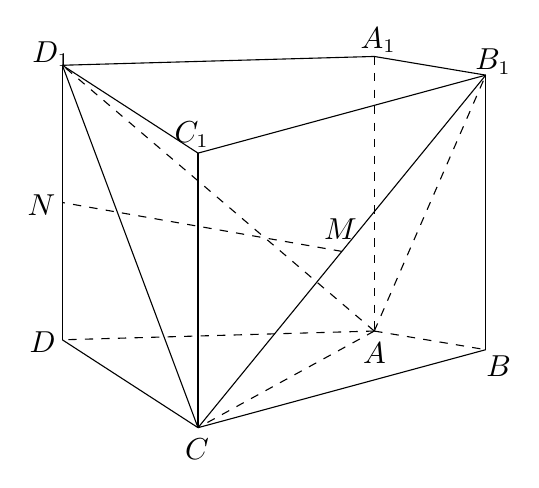
\begin{tikzpicture}[
  x=1pt,y=1pt,                             % 画布单位 = 1 pt（本文件坐标一律为 pt）
  every node/.style={font=\fontsize{10.5pt}{12.6pt}\selectfont,inner sep=0pt},
  s/.style={line width=0.3985pt},
  d/.style={line width=0.3985pt,dash pattern=on 2.98883pt off 2.98883pt},
]

  % ---------- 实线 11 条 ----------
  \draw[s] (0.00,130.96) -- (0.00,31.75);       % 1  D₁D
  \draw[s] (49.02,99.21) -- (49.02,0.00);       % 2  C₁C
  \draw[s] (112.71,134.14) -- (152.99,127.39);  % 3  A₁B₁
  \draw[s] (152.99,127.39) -- (49.02,99.21);    % 4  B₁C₁
  \draw[s] (49.02,99.21) -- (0.00,130.96);      % 5  C₁D₁
  \draw[s] (0.00,130.96) -- (112.71,134.14);    % 6  D₁A₁
  \draw[s] (49.02,0.00) -- (0.00,130.96);       % 7  D₁C
  \draw[s] (49.02,0.00) -- (152.99,127.39);     % 8  B₁C
  \draw[s] (152.99,127.39) -- (152.99,28.18);   % 9  B₁B
  \draw[s] (0.00,31.75) -- (49.02,0.00);        % 10 DC
  \draw[s] (49.02,0.00) -- (152.99,28.18);      % 11 CB

  % ---------- 虚线 7 条 ----------
  \draw[d] (112.71,134.14) -- (112.71,34.92);   % 12 A₁A
  \draw[d] (112.71,34.92) -- (152.99,28.18);    % 13 AB
  \draw[d] (112.71,34.92) -- (49.02,0.00);      % 14 AC
  \draw[d] (112.71,34.92) -- (0.00,31.75);      % 15 AD
  \draw[d] (112.71,34.92) -- (152.99,127.39);   % 16 AB₁
  \draw[d] (112.71,34.92) -- (0.00,130.96);     % 17 AD₁
  \draw[d] (101.01,63.70) -- (0.00,81.36);      % 18 NM（M → N）

  % ---------- 标签（清单 §4.1 / §4.3 实测字形中心）----------
  \node at (-4.04,134.98)  {$D_1$};
  \node at (114.16,139.98) {$A_1$};
  \node at (155.66,132.18) {$B_1$};
  \node at (46.76,105.98)  {$C_1$};
  \node at (-7.14,30.78)   {$D$};
  \node at (112.76,26.98)  {$A$};
  \node at (157.66,22.28)  {$B$};
  \node at (48.66,-7.92)   {$C$};
  \node at (-7.54,80.38)   {$N$};
  \node at (100.46,71.68)  {$M$};

\end{tikzpicture}
\end{center}
\nopagebreak[4]
（1） 求证：\(MN\parallel\) 平面 \(ABCD\)；

（2） 求二面角 \(D_1\text{-}AC\text{-}B_1\) 的正弦值；

（3） 设 \(E\) 为棱 \(A_1B_1\) 上的点，若直线 \(NE\) 和平面 \(ABCD\) 所成角的正弦值为 \(\dfrac{1}{3}\)，求线段 \(A_1E\) 的长．

\Needspace{4\baselineskip}
\textbf{解析}

侧棱 \(A_{1}A\perp\) 底面 \(ABCD\)，又 \(AB\perp AC\)，故以 \(A\) 为原点、\(\overrightarrow{AB}\)、\(\overrightarrow{AC}\)、\(\overrightarrow{AA_{1}}\) 为三条坐标轴建立空间直角坐标系，平行、二面角、线面角三类问题一并化为向量运算。

\gksubpart{(1)}

\Needspace{5\baselineskip}
建系后 \(A(0,0,0)\)，\(B(1,0,0)\)，\(C(0,2,0)\)。由 \(AD=CD=\sqrt{5}\) 知 \(D\) 在 \(AC\) 的中垂线 \(y=1\) 上，设 \(D(x_{0},1,0)\)，由 \(x_{0}^{2}+1=5\) 得 \(x_{0}=\pm2\)；其中 \(x_{0}=2\) 使四边形 \(ABCD\) 非凸，与棱柱底面为凸四边形矛盾，故取 \(D(-2,1,0)\)。又 \(AA_{1}=2\) 且垂直于底面，得 \(B_{1}(1,0,2)\)，\(D_{1}(-2,1,2)\)。而 \(M\)、\(N\) 分别为 \(B_{1}C\)、\(D_{1}D\) 的中点，故
\nopagebreak[4]
\[
M\left(\dfrac{1}{2},1,1\right),\qquad N(-2,1,1),
\]
\nopagebreak[4]
\[
\overrightarrow{MN}=\left(-\dfrac{5}{2},0,0\right).
\]
\(\overrightarrow{MN}\) 的 \(z\) 分量为 0，即 \(\overrightarrow{MN}\perp(0,0,1)\)，而 \((0,0,1)\) 是底面 \(ABCD\) 的法向量，故 \(MN\parallel\) 平面 \(ABCD\)；又 \(M\) 的 \(z\) 坐标为 1，不在底面内，所以 \(MN\) 平行于平面而不落在平面内。从图形上看，\(M\)、\(N\) 分别是两条斜线段的中点，二者相对于底面的高度相同（\(z\) 坐标同为 1），故 \(MN\) 沿水平方向延伸，与底面平行。

\gksubpart{(2)}

\Needspace{5\baselineskip}
\(\overrightarrow{AB_{1}}=(1,0,2)\)，\(\overrightarrow{AC}=(0,2,0)\)，\(\overrightarrow{AD_{1}}=(-2,1,2)\)。面 \(ACB_{1}\) 的法向量
\nopagebreak[4]
\[
\vec{n}_{1}=\overrightarrow{AB_{1}}\times\overrightarrow{AC}=(-4,0,2),
\]
\Needspace{5\baselineskip}
面 \(ACD_{1}\) 的法向量
\nopagebreak[4]
\[
\vec{n}_{2}=\overrightarrow{AD_{1}}\times\overrightarrow{AC}=(-4,0,-4).
\]
\Needspace{5\baselineskip}
设二面角 \(D_{1}-AC-B_{1}\) 的大小为 \(\theta\)，则
\nopagebreak[4]
\[
\cos\theta=\dfrac{\left|\vec{n}_{1}\cdot\vec{n}_{2}\right|}{\left|\vec{n}_{1}\right|\left|\vec{n}_{2}\right|}
=\dfrac{16-8}{2\sqrt{5}\times4\sqrt{2}}=\dfrac{8}{8\sqrt{10}}=\dfrac{1}{\sqrt{10}},
\]
\nopagebreak[4]
\[
\sin\theta=\sqrt{1-\dfrac{1}{10}}=\dfrac{3}{\sqrt{10}}=\dfrac{3\sqrt{10}}{10}.
\]

另可用垂足法一句话核对：由 \(AC\perp AB\) 且 \(AC\perp AA_{1}\) 得 \(AC\perp\) 平面 \(ABB_{1}A_{1}\)，从而 \(AC\perp AB_{1}\)；\(D_{1}\) 在 \(AC\) 上的射影为 \(AC\) 的中点 \(F_{0}(0,1,0)\)，于是 \(\overrightarrow{AB_{1}}\) 与 \(\overrightarrow{F_{0}D_{1}}\) 都垂直于 \(AC\)，二者夹角即二面角的平面角，由 \(\overrightarrow{AB_{1}}\cdot\overrightarrow{F_{0}D_{1}}=2\)、\(\left|\overrightarrow{AB_{1}}\right|=\sqrt{5}\)、\(\left|\overrightarrow{F_{0}D_{1}}\right|=2\sqrt{2}\) 得 \(\cos\theta=\dfrac{2}{2\sqrt{10}}=\dfrac{1}{\sqrt{10}}\)，与法向量法结论一致。

\gksubpart{(3)}

\Needspace{5\baselineskip}
设 \(A_{1}E=t\)（\(0\leqslant t\leqslant1\)），则 \(E(t,0,2)\)；又 \(N(-2,1,1)\)，故
\nopagebreak[4]
\[
\overrightarrow{NE}=(t+2,-1,1),\qquad \left|\overrightarrow{NE}\right|=\sqrt{(t+2)^{2}+2}.
\]
\Needspace{5\baselineskip}
底面 \(ABCD\) 的法向量为 \((0,0,1)\)，设直线 \(NE\) 与底面所成角为 \(\varphi\)，则
\nopagebreak[4]
\[
\sin\varphi=\dfrac{\left|\overrightarrow{NE}\cdot(0,0,1)\right|}{\left|\overrightarrow{NE}\right|}
=\dfrac{1}{\sqrt{(t+2)^{2}+2}}=\dfrac{1}{3},
\]
\Needspace{5\baselineskip}
即 \((t+2)^{2}+2=9\)，\((t+2)^{2}=7\)，解得 \(t=\sqrt{7}-2\) 或 \(t=-\sqrt{7}-2\)；后者为负值，舍去。\(\sqrt{7}-2\approx0.646\in[0,1]\)，符合 \(E\) 在棱 \(A_{1}B_{1}\) 上，故
\nopagebreak[4]
\[
A_{1}E=\sqrt{7}-2 .
\]

（验证：建系数据复核 \(AB=1\)、\(AC=2\)、\(AD=CD=\sqrt{5}\)、\(\overrightarrow{AB}\cdot\overrightarrow{AC}=0\) 全部符合题设；底面取 \(D(-2,1,0)\) 时四顶点同向（凸），另一解 \(D(2,1,0)\) 判为非凸而舍去，故 \(D\) 的取法唯一。(2) 三种独立算法同值 \(\sin\theta=0.948683298051=\dfrac{3\sqrt{10}}{10}\)：法向量夹角法、垂足法（垂足 \(F_{0}=(0,1,0)\)）与点面距法（\(D_{1}\) 到平面 \(ACB_{1}\) 的距离 \(2.683281573000\) 与 \(|D_{1}F_{0}|=2.828427124746\) 之比）。(3) 把 \(A_{1}E=\sqrt{7}-2=0.645751311\) 回代得 \(\left|\overrightarrow{NE}\right|=3.000000000\)、\(\sin\varphi=0.333333333=\dfrac{1}{3}\)；而 \(A_{1}E\) 取 \(0,0.5,1\) 时对应的正弦值为 \(0.408,0.348,0.302\)，均不等于 \(\dfrac{1}{3}\)，故解唯一。）

\gkanswer{答案（1）：成立（建系后 \(\overrightarrow{MN}=\left(-\dfrac52,0,0\right)\) 与底面法向量垂直、\(z\) 分量为 0，即 \(MN\parallel\) 平面；又 \(M\notin\) 平面 \(ABCD\)，故 \(MN\parallel\) 平面 \(ABCD\)）。}

\gkanswer{答案（2）：\(\dfrac{3\sqrt{10}}{10}\)。}

\gkanswer{答案（3）：\(\sqrt{7}-2\)。}

\end{answer}
\begin{answer}
\gksolhead{18}{}

\textbf{题目}：

已知数列 \(\{a_n\}\) 满足 \(a_{n+2}=qa_n\)（\(q\) 为实数，且 \(q\neq1\)），\(n\in\mathbf{N}^{*}\)，\(a_1=1\)，\(a_2=2\)，且 \(a_2+a_3\)，\(a_3+a_4\)，\(a_4+a_5\) 成等差数列．

（1） 求 \(q\) 的值和 \(\{a_n\}\) 的通项公式；

（2） 设 \(b_n=\dfrac{\log_2 a_{2n}}{a_{2n-1}}\)，\(n\in\mathbf{N}^{*}\)，求数列 \(\{b_n\}\) 的前 \(n\) 项和．

\Needspace{4\baselineskip}
\textbf{解析}

递推式 \(a_{n+2}=qa_{n}\) 表明奇数项、偶数项各自成公比为 \(q\) 的等比数列，先用等差条件确定 \(q\)，写出通项后代出 \(b_{n}\)，再用错位相减求和。

\gksubpart{(1)}

由 \(a_{n+2}=qa_{n}\) 及 \(a_{1}=1\)、\(a_{2}=2\)：奇数项 \(a_{1}=1\)，\(a_{3}=q\)，\(a_{5}=q^{2}\)，\(\dots\)，即 \(a_{2k-1}=q^{k-1}\)；偶数项 \(a_{2}=2\)，\(a_{4}=2q\)，\(a_{6}=2q^{2}\)，\(\dots\)，即 \(a_{2k}=2q^{k-1}\)。

\Needspace{5\baselineskip}
\(a_{2}+a_{3}\)，\(a_{3}+a_{4}\)，\(a_{4}+a_{5}\) 成等差数列，等价于
\nopagebreak[4]
\[
(a_{2}+a_{3})+(a_{4}+a_{5})=2(a_{3}+a_{4}),
\]
\Needspace{5\baselineskip}
即 \(a_{2}+a_{5}=a_{3}+a_{4}\)，代入得
\nopagebreak[4]
\[
2+q^{2}=q+2q \Longrightarrow q^{2}-3q+2=0,
\]
解得 \(q=1\) 或 \(q=2\)，由 \(q\neq1\) 得 \(q=2\)。

\Needspace{5\baselineskip}
于是通项分奇偶写出：\(a_{n}=2^{\frac{n-1}{2}}\)（\(n\) 为奇数），\(a_{n}=2^{\frac{n}{2}}\)（\(n\) 为偶数），即数列为
\nopagebreak[4]
\[
1,\ 2,\ 2,\ 4,\ 4,\ 8,\ 8,\ \dots
\]

\gksubpart{(2)}

\Needspace{5\baselineskip}
由通项，\(a_{2n}=2^{n}\)，\(a_{2n-1}=2^{n-1}\)，故
\nopagebreak[4]
\[
b_{n}=\dfrac{\log_{2}a_{2n}}{a_{2n-1}}=\dfrac{n}{2^{\,n-1}} .
\]
\Needspace{5\baselineskip}
记 \(S_{n}=\sum\limits_{k=1}^{n}\dfrac{k}{2^{\,k-1}}\)，则 \(\dfrac{1}{2}S_{n}=\sum\limits_{k=1}^{n}\dfrac{k}{2^{\,k}}\)，两式错位相减：
\nopagebreak[4]
\[
\dfrac{1}{2}S_{n}=1+\left(\dfrac{1}{2}+\dfrac{1}{2^{2}}+\dots+\dfrac{1}{2^{\,n-1}}\right)-\dfrac{n}{2^{\,n}}
=1+\left(1-\dfrac{1}{2^{\,n-1}}\right)-\dfrac{n}{2^{\,n}}
=2-\dfrac{1}{2^{\,n-1}}-\dfrac{n}{2^{\,n}},
\]
\Needspace{5\baselineskip}
其中括号内是首项为 \(\dfrac{1}{2}\)、公比为 \(\dfrac{1}{2}\)、共 \(n-1\) 项的等比数列之和。于是
\nopagebreak[4]
\[
S_{n}=2\left(2-\dfrac{1}{2^{\,n-1}}-\dfrac{n}{2^{\,n}}\right)
=4-\dfrac{2}{2^{\,n-1}}-\dfrac{n}{2^{\,n-1}}=4-\dfrac{n+2}{2^{\,n-1}} .
\]

（验证：由 \(a_{1}=1\)、\(a_{2}=2\)、\(q=2\) 生成的数列 \(1,2,2,4,4,8,8,\dots\) 对 \(n\leqslant40\) 逐项检验递推关系 \(a_{n+2}=2a_{n}\) 全部成立；等差条件的三数和为 \(4,6,8\)，满足 \(2\times6=4+8\)；\(b_{n}\) 的定义式与 \(\dfrac{n}{2^{\,n-1}}\) 对 \(n\leqslant20\) 数值恒等；求和公式与分数精确的逐项直接求和 \(n=1,2,\dots,12\) 完全相等，两端点核对 \(S_{1}=1=b_{1}\)、\(S_{3}=\dfrac{11}{4}=1+1+\dfrac{3}{4}\)，且 \(n\to\infty\) 时 \(S_{n}\to4\)，与 \(\sum\limits_{k=1}^{\infty}\dfrac{k}{2^{\,k-1}}\) 的理论极限一致。）

\gkanswer{答案（1）：\(q=2\)，\(a_n=2^{\frac{n-1}{2}}\)（\(n\) 为奇数时），\(a_n=2^{\frac{n}{2}}\)（\(n\) 为偶数时）。}

\gkanswer{答案（2）：\(S_n=4-\dfrac{n+2}{2^{n-1}}\)。}

\end{answer}
\begin{answer}
\gksolhead{19}{}

\textbf{题目}：

已知椭圆 \(\dfrac{x^2}{a^2}+\dfrac{y^2}{b^2}=1\)（\(a>b>0\)）的左焦点为 \(F(-c,0)\)，离心率为 \(\dfrac{\sqrt{3}}{3}\)，点 \(M\) 在椭圆上且位于第一象限，直线 \(FM\) 被圆 \(x^2+y^2=\dfrac{b^2}{4}\) 截得的线段的长为 \(c\)，\(|FM|=\dfrac{4\sqrt{3}}{3}\)．

（1） 求直线 \(FM\) 的斜率；

（2） 求椭圆的方程；

（3） 设动点 \(P\) 在椭圆上，若直线 \(FP\) 的斜率大于 \(\sqrt{2}\)，求直线 \(OP\)（\(O\) 为原点）的斜率的取值范围．

\Needspace{4\baselineskip}
\textbf{解析}

由离心率把 \(c^{2}\)、\(b^{2}\) 都化成 \(a^{2}\) 的倍比，弦长条件给出斜率 \(k\) 的方程；再由 \(|FM|\) 与点 \(M\) 的位置定出 \(a\)；第 (3) 问以直线 \(FP\) 的斜率为参数，把满足条件的点分为上、下两支弧，分别求 \(k_{OP}\) 的取值范围。

\gksubpart{(1)}

\Needspace{5\baselineskip}
由 \(e=\dfrac{c}{a}=\dfrac{\sqrt{3}}{3}\) 得 \(c=\dfrac{a}{\sqrt{3}}\)，从而
\nopagebreak[4]
\[
b^{2}=a^{2}-c^{2}=\dfrac{2}{3}a^{2},
\]
圆 \(x^{2}+y^{2}=\dfrac{b^{2}}{4}\) 的半径 \(r=\dfrac{b}{2}\)。

\Needspace{5\baselineskip}
点 \(M\) 在第一象限，故直线 \(FM\) 的斜率 \(k>0\)，方程可写为 \(y=k(x+c)\)，即 \(kx-y+kc=0\)，原点 \(O\) 到它的距离
\nopagebreak[4]
\[
d=\dfrac{kc}{\sqrt{1+k^{2}}} .
\]
\Needspace{5\baselineskip}
该直线被圆截得的弦长恰为 \(c\)，由弦长公式 \(c=2\sqrt{r^{2}-d^{2}}\) 得
\nopagebreak[4]
\[
r^{2}-d^{2}=\dfrac{c^{2}}{4}.
\]
\Needspace{5\baselineskip}
代入 \(r^{2}=\dfrac{b^{2}}{4}=\dfrac{a^{2}}{6}\)、\(c^{2}=\dfrac{a^{2}}{3}\)，得 \(d^{2}=\dfrac{a^{2}}{6}-\dfrac{a^{2}}{12}=\dfrac{a^{2}}{12}\)；又
\nopagebreak[4]
\[
d^{2}=\dfrac{k^{2}c^{2}}{1+k^{2}}=\dfrac{k^{2}a^{2}}{3(1+k^{2})},
\]
\Needspace{5\baselineskip}
于是
\nopagebreak[4]
\[
\dfrac{k^{2}}{3(1+k^{2})}=\dfrac{1}{12} \Longrightarrow 12k^{2}=3+3k^{2} \Longrightarrow 9k^{2}=3 \Longrightarrow k^{2}=\dfrac{1}{3},
\]
由 \(k>0\) 得 \(k=\dfrac{\sqrt{3}}{3}\)。

\gksubpart{(2)}

\Needspace{5\baselineskip}
\(k=\dfrac{\sqrt{3}}{3}\) 时直线 \(FM\) 的倾斜角为 \(30^{\circ}\)，\(\cos\theta=\dfrac{\sqrt{3}}{2}\)，\(\sin\theta=\dfrac{1}{2}\)。由 \(|FM|=\dfrac{4\sqrt{3}}{3}\) 得
\nopagebreak[4]
\[
M=\left(-c+\dfrac{4\sqrt{3}}{3}\times\dfrac{\sqrt{3}}{2},\ \dfrac{4\sqrt{3}}{3}\times\dfrac{1}{2}\right)=\left(2-c,\ \dfrac{2\sqrt{3}}{3}\right).
\]
\Needspace{5\baselineskip}
点 \(M\) 在椭圆上，代入 \(\dfrac{x^{2}}{a^{2}}+\dfrac{y^{2}}{b^{2}}=1\) 并利用 \(c=\dfrac{a}{\sqrt{3}}\)、\(b^{2}=\dfrac{2a^{2}}{3}\)：
\nopagebreak[4]
\[
\dfrac{\left(2-\dfrac{a}{\sqrt{3}}\right)^{2}}{a^{2}}+\dfrac{\dfrac{4}{3}}{\dfrac{2a^{2}}{3}}=1 \Longrightarrow \left(2-\dfrac{a}{\sqrt{3}}\right)^{2}+2=a^{2},
\]
\nopagebreak[4]
\[
\Longrightarrow 6-\dfrac{4a}{\sqrt{3}}+\dfrac{a^{2}}{3}=a^{2} \Longrightarrow a^{2}+2\sqrt{3}\,a-9=0,
\]
\Needspace{5\baselineskip}
解得 \(a=\dfrac{-2\sqrt{3}+\sqrt{12+36}}{2}=\sqrt{3}\)（负根 \(-3\sqrt{3}\) 舍去）。于是 \(a^{2}=3\)，\(c=1\)，\(b^{2}=2\)，椭圆方程为
\nopagebreak[4]
\[
\dfrac{x^{2}}{3}+\dfrac{y^{2}}{2}=1,
\]
此时 \(M\left(1,\dfrac{2\sqrt{3}}{3}\right)\) 确在第一象限。

\gksubpart{(3)}

\Needspace{5\baselineskip}
设 \(P(x,y)\) 为椭圆上满足条件的点，条件即 \(k_{FP}=\dfrac{y}{x+1}>\sqrt{2}\)，并要求 \(x\neq-1\)。对每个 \(m>\sqrt{2}\)，直线 \(y=m(x+1)\) 过左焦点 \(F(-1,0)\)，而 \(F\) 在椭圆内部（\(\dfrac{1}{3}+0<1\)），故该直线与椭圆恰有两个交点，且这两个交点都满足 \(k_{FP}=m>\sqrt{2}\)。代入椭圆方程得
\nopagebreak[4]
\[
(2+3m^{2})x^{2}+6m^{2}x+3m^{2}-6=0,
\]
两根分别落在上支（\(y>0\)，\(x\in(-1,0)\)）与下支（\(y<0\)，\(x\in\left(-\dfrac{3}{2},-1\right)\)）上。

\Needspace{5\baselineskip}
① 上支：\(m=\sqrt{2}\) 时交点为 \((0,\sqrt{2})\)，但 \(m>\sqrt{2}\) 是严格不等，该点应挖去；\(m\to+\infty\) 时上支交点趋于 \(\left(-1,\dfrac{2\sqrt{3}}{3}\right)\)，此处 \(FP\) 竖直、斜率不存在，也应挖去。弧上
\nopagebreak[4]
\[
k_{OP}=\dfrac{y}{x}=-\dfrac{\sqrt{2-\dfrac{2x^{2}}{3}}}{|x|}\qquad(-1<x<0),
\]
\Needspace{5\baselineskip}
它随 \(x\) 由 \(-1\) 增至 \(0\) 严格递减，取值从 \(-\dfrac{2\sqrt{3}}{3}\) 一直降到 \(-\infty\)；两端点均已挖去，故
\nopagebreak[4]
\[
k_{OP}\in\left(-\infty,-\dfrac{2\sqrt{3}}{3}\right).
\]

② 下支：\(m=\sqrt{2}\) 时交点为 \(\left(-\dfrac{3}{2},-\dfrac{\sqrt{2}}{2}\right)\)，应挖去。

\Needspace{5\baselineskip}
\(m\to+\infty\) 时交点趋于 \(\left(-1,-\dfrac{2\sqrt{3}}{3}\right)\)，也应挖去。弧上
\nopagebreak[4]
\[
k_{OP}=\dfrac{\sqrt{2-\dfrac{2x^{2}}{3}}}{|x|}\qquad\left(-\dfrac{3}{2}<x<-1\right),
\]
\Needspace{5\baselineskip}
它随 \(x\) 增大严格递增，取值从 \(\dfrac{\sqrt{2}}{3}\) 增到 \(\dfrac{2\sqrt{3}}{3}\)，两端点挖去，故
\nopagebreak[4]
\[
k_{OP}\in\left(\dfrac{\sqrt{2}}{3},\dfrac{2\sqrt{3}}{3}\right).
\]

\Needspace{5\baselineskip}
综上，直线 \(OP\) 的斜率的取值范围为
\nopagebreak[4]
\[
\left(-\infty,-\dfrac{2\sqrt{3}}{3}\right)\cup\left(\dfrac{\sqrt{2}}{3},\dfrac{2\sqrt{3}}{3}\right).
\]

存疑登记：以上按题面字面理解，凡使 \(k_{FP}>\sqrt{2}\) 的点（上、下两支）都计入；若命题本意是限定点 \(P\) 在第二象限（只保留上支），则取值范围缩为 \(\left(-\infty,-\dfrac{2\sqrt{3}}{3}\right)\)。

（验证：(1) 以 \(k=\dfrac{\sqrt{3}}{3}\)、\(c=1\) 独立复算：圆心距 \(d=\dfrac{kc}{\sqrt{1+k^{2}}}=0.500000\)、圆半径 \(r=\dfrac{b}{2}=0.707107\)，弦长 \(2\sqrt{r^{2}-d^{2}}=1.000000=c\)，与题设自洽；(2) 精确分数代入 \(a=\sqrt{3}=1.732050807569\)、\(c=1.000000\)、\(b^{2}=2.000000\)，点 \(M=(1,1.154700538)\) 代入椭圆左端得 \(1.000000000000\)，且独立算得 \(|FM|=\sqrt{2^{2}+\left(\dfrac{2\sqrt{3}}{3}\right)^{2}}=2.309401=\dfrac{4\sqrt{3}}{3}\)，\(M\) 确在第一象限；(3) 对 \(m=\sqrt{2},1.5,1.6,2,3,5,10,30,100,10^{3},10^{6}\) 两支逐点扫描：每个交点的 \(FP\) 斜率恰等于所设 \(m\)，上支 \(k_{OP}\) 由 \(-24.49\) 严格递增到 \(-1.15470\)，下支由 \(0.4714\) 严格递增到 \(1.1527\)；端点极限值与解析端点 \(-\dfrac{2\sqrt{3}}{3}=-1.154700538\)、\(\dfrac{\sqrt{2}}{3}=0.471404521\)、\(\dfrac{2\sqrt{3}}{3}=1.154700538\) 吻合。）

\gkanswer{答案（1）：\(\dfrac{\sqrt{3}}{3}\)。}

\gkanswer{答案（2）：\(\dfrac{x^2}{3}+\dfrac{y^2}{2}=1\)。}

\gkanswer{答案（3）：\(\left(-\infty,-\dfrac{2\sqrt{3}}{3}\right)\cup\left(\dfrac{\sqrt{2}}{3},\dfrac{2\sqrt{3}}{3}\right)\)。}

\end{answer}
\begin{answer}
\gksolhead{20}{}

\textbf{题目}：

已知函数 \(f(x)=nx-x^n\)，\(x\in\mathbf{R}\)，其中 \(n\in\mathbf{N}^{*}\)，且 \(n\geqslant2\)．

（1） 讨论 \(f(x)\) 的单调性；

（2） 设曲线 \(y=f(x)\) 与 \(x\) 轴正半轴的交点为 \(P\)，曲线在点 \(P\) 处的切线方程为 \(y=g(x)\)，求证：对于任意的正实数 \(x\)，都有 \(f(x)\leqslant g(x)\)；

（3） 若关于 \(x\) 的方程 \(f(x)=a\)（\(a\) 为实数）有两个正实数根 \(x_1\)，\(x_2\)，求证：\(|x_2-x_1|<\dfrac{a}{1-n}+2\)．

\Needspace{4\baselineskip}
\textbf{解析}

\(f'(x)=n\left(1-x^{\,n-1}\right)\) 的符号由 \(x^{\,n-1}\) 与 \(1\) 的大小决定，而 \(x^{\,n-1}\) 的增减性随 \(n\) 的奇偶而不同，故 (1) 必须分奇偶讨论；(2) 把 \(f\leqslant g\) 化归为辅助函数 \(h=g-f\) 的最小值问题；(3) 用切线不等式与 \(x_{1}>\dfrac{a}{n}\) 两条严格界相减放缩。

\gksubpart{(1)}

\nopagebreak[4]
\[
f'(x)=n-nx^{\,n-1}=n\left(1-x^{\,n-1}\right)\qquad(n\in\mathbf{N}^{*},\ n\geqslant2).
\]

① 当 \(n\) 为偶数时，\(n-1\) 为奇数，\(x^{\,n-1}\) 在 \(\mathbf{R}\) 上递增，\(x^{\,n-1}<1\) 等价于 \(x<1\)，故 \(f(x)\) 在 \((-\infty,1)\) 上单调递增，在 \((1,+\infty)\) 上单调递减；

② 当 \(n\) 为奇数时，\(n-1\) 为偶数，\(x^{\,n-1}=|x|^{\,n-1}\)，\(x^{\,n-1}<1\) 等价于 \(|x|<1\)，故 \(f(x)\) 在 \((-1,1)\) 上单调递增，在 \((-\infty,-1)\) 与 \((1,+\infty)\) 上单调递减。

两种情形下 \(f\) 都在 \(x=1\) 处取最大值 \(f(1)=n-1\)；且在正半轴上单调性统一：\((0,1)\) 上递增，\((1,+\infty)\) 上递减。

\gksubpart{(2)}

\Needspace{5\baselineskip}
曲线 \(y=f(x)\) 与 \(x\) 轴正半轴的交点 \(P\) 满足 \(nx=x^{n}\)，即 \(x^{\,n-1}=n\)，故
\nopagebreak[4]
\[
t=x_{P}=n^{\frac{1}{n-1}},
\]
\Needspace{5\baselineskip}
即 \(P(t,0)\)，且 \(f'(t)=n\left(1-t^{\,n-1}\right)=n(1-n)\)。曲线在点 \(P\) 处的切线为
\nopagebreak[4]
\[
g(x)=f'(t)(x-t)=n(1-n)(x-t).
\]
\Needspace{5\baselineskip}
令 \(h(x)=g(x)-f(x)\)，则
\nopagebreak[4]
\[
h(x)=n(1-n)(x-t)-nx+x^{n}=x^{n}-n^{2}x+n(n-1)t,
\]
\nopagebreak[4]
\[
h'(x)=nx^{\,n-1}-n^{2}=n\left(x^{\,n-1}-t^{\,n-1}\right).
\]
\Needspace{5\baselineskip}
当 \(x>0\) 时 \(x^{\,n-1}\) 随 \(x\) 严格递增，故 \(h\) 在 \((0,t)\) 上递减、在 \((t,+\infty)\) 上递增，于 \(x=t\) 处取最小值：
\nopagebreak[4]
\[
h(t)=t^{n}-n^{2}t+n(n-1)t=t\times t^{\,n-1}-n^{2}t+n(n-1)t=tn-n^{2}t+n^{2}t-nt=0 .
\]
\Needspace{5\baselineskip}
所以对任意正实数 \(x\) 都有 \(h(x)\geqslant0\)，即
\nopagebreak[4]
\[
f(x)\leqslant g(x),
\]
等号当且仅当 \(x=t\)。

\gksubpart{(3)}

\Needspace{5\baselineskip}
由 (1)，\(f\) 在 \((0,1)\) 上从 \(0\) 递增到 \(n-1\)，在 \((1,t)\) 上从 \(n-1\) 递减到 \(0\)（\(t=n^{\frac{1}{n-1}}\) 是 \(f\) 在正半轴上的另一个零点）。又因
\nopagebreak[4]
\[
2^{\,n-1}=(1+1)^{\,n-1}\geqslant1+(n-1)=n,
\]
\Needspace{5\baselineskip}
故 \(t=n^{\frac{1}{n-1}}\leqslant2\)。于是方程 \(f(x)=a\) 有两个正实根当且仅当 \(0<a<n-1\)，且此时
\nopagebreak[4]
\[
0<x_{1}<1<x_{2}<t .
\]

\Needspace{5\baselineskip}
① 在 \(x=x_{2}\) 处用 \(f(x)\leqslant g(x)\) 得
\nopagebreak[4]
\[
a=f(x_{2})\leqslant g(x_{2})=n(1-n)(x_{2}-t),
\]
\Needspace{5\baselineskip}
由 \(n(1-n)<0\)，两边同除以 \(n(1-n)\) 得 \(x_{2}-t\leqslant\dfrac{a}{n(1-n)}=-\dfrac{a}{n(n-1)}\)，即
\nopagebreak[4]
\[
t-x_{2}\geqslant\dfrac{a}{n(n-1)} ;
\]
等号当且仅当 \(x_{2}=t\)，而 \(x_{2}<t\)，故此不等式严格成立：\(t-x_{2}>\dfrac{a}{n(n-1)}\)。

\Needspace{5\baselineskip}
② 由 \(a=nx_{1}-x_{1}^{\,n}<nx_{1}\)（因 \(x_{1}>0\)）得
\nopagebreak[4]
\[
x_{1}>\dfrac{a}{n},
\]
同样严格。

\Needspace{5\baselineskip}
将两式相减：由 \(x_{2}-x_{1}=(t-x_{1})-(t-x_{2})\)，其中 \(t-x_{1}\) 用 ② 的上界、\(t-x_{2}\) 用 ① 的下界，得
\nopagebreak[4]
\[
x_{2}-x_{1}<\left(t-\dfrac{a}{n}\right)-\dfrac{a}{n(n-1)}
=t-\dfrac{a}{n}-\dfrac{a}{n(n-1)}=t-\dfrac{a}{n-1}\leqslant2-\dfrac{a}{n-1}=\dfrac{a}{1-n}+2,
\]
\Needspace{5\baselineskip}
即
\nopagebreak[4]
\[
\left|x_{2}-x_{1}\right|<\dfrac{a}{1-n}+2 .
\]

（验证：(1) 分奇偶逐点验证：\(n=2,4\) 时在 \((-\infty,1)\) 上递增、在 \((1,+\infty)\) 上递减，\(n=3,5\) 时在 \((-\infty,-1)\) 上递减、在 \((-1,1)\) 上递增、在 \((1,+\infty)\) 上递减，全部成立；若把偶数情形的结论照搬到奇数 \(n\)，会被 \(f(-6)=198>f(-1)=-2\) 立即否掉，可见分奇偶讨论不可省。(2) 在 \((0,5]\) 上取 4 万点扫描 \(\min(g-f)\)，\(n=2,3,4,7\) 分别得 \(0\)、\(1.3\times10^{-8}\)、\(1.0\times10^{-8}\)、\(1.5\times10^{-7}\)，均不小于 0，\(f(t)\) 与 0 的偏差在 \(10^{-15}\) 量级。(3) 用二分法求出精确根后，对 \(n\in\{2,3,4,6,10\}\) 与 \(a\in\{0.001,\ 0.1,\ 0.5,\ 0.9(n-1),\ 0.999(n-1)\}\) 共 25 组逐组核对 \(\left|x_{2}-x_{1}\right|<\dfrac{a}{1-n}+2\) 全部成立，其中最紧的一组 \(n=2\)、\(a=0.001\) 仍有裕度 \(2.5\times10^{-7}\)，\(n\geqslant3\) 时裕度稳定在 \(0.27\) 与 \(0.97\) 之间；证明所用的两条界 \(t-x_{2}>\dfrac{a}{n(n-1)}\) 与 \(x_{1}>\dfrac{a}{n}\) 在 \((n,a)=(2,0.5),(3,1),(5,2)\) 三处也逐一复核成立。）

\gkanswer{答案（1）：当 \(n\) 为偶数时，\(f(x)\) 在 \((-\infty,1)\) 上单调递增、在 \((1,+\infty)\) 上单调递减；当 \(n\) 为奇数时，\(f(x)\) 在 \((-\infty,-1)\) 上单调递减、在 \((-1,1)\) 上单调递增、在 \((1,+\infty)\) 上单调递减。}

\gkanswer{答案（2）：成立（记 \(t=n^{\frac{1}{n-1}}\)，\(P(t,0)\)；切线 \(g(x)=n(1-n)(x-t)\)，令 \(h=g-f=x^n-n^2x+n(n-1)t\)，则 \(h'=n\left(x^{n-1}-t^{n-1}\right)\)，\(h\) 在 \(x=t\) 取最小值 \(h(t)=0\)，故对任意正实数 \(x\) 有 \(h\geqslant0\)，等号仅当 \(x=t\)）。}

\gkanswer{答案（3）：成立（记 \(t=n^{\frac{1}{n-1}}\leqslant2\)，等号仅 \(n=2\)；由切线不等式得严格界 \(t-x_2\geqslant\dfrac{a}{n(n-1)}\)，又 \(x_1>\dfrac{a}{n}\)（严格），相减得 \(x_2-x_1<t-\dfrac{a}{n-1}\leqslant2-\dfrac{a}{n-1}=\dfrac{a}{1-n}+2\)）。}

\end{answer}